\section{Откуда берутся датасеты}

\begin{frame}[c]{Откуда берутся данные}
  \begin{columns}[T]
    \begin{column}{0.23\textwidth}
      \begin{block}{Готовые}
        \small
        Kaggle, Hugging Face, UCI. Быстро, но задачу за вас уже кто-то сформулировал.
      \end{block}
    \end{column}
    \begin{column}{0.23\textwidth}
      \begin{block}{Собранные}
        \small
        Логи сервиса, парсинг сайтов, датчики, фото на телефон.
      \end{block}
    \end{column}
    \begin{column}{0.23\textwidth}
      \begin{block}{Размеченные}
        \small
        Объекты есть, ответов нет. Ответы ставят люди: эксперты или краудсорсинг.
      \end{block}
    \end{column}
    \begin{column}{0.23\textwidth}
      \begin{block}{Синтетические}
        \small
        Сгенерированы по формуле или другой моделью.
      \end{block}
    \end{column}
  \end{columns}

  \medskip
  \lead{Чаще всего самое долгое в ML-проекте --- не обучение, а сбор и чистка данных.}
\end{frame}

\begin{frame}[c]{MNIST: рукописные цифры}
  \begin{columns}[T]
    \begin{column}{0.50\textwidth}
      \centering
      % Handwritten digits 8x8 from the UCI Optical Recognition of Handwritten Digits
% dataset (copy shipped with scikit-learn, digits.csv.gz). Two samples per digit.
\begin{tikzpicture}[x=0.075cm,y=0.075cm]
  \fill[acLight] (0.0,0.0) rectangle ++(8,-8);
  \fill[acDark!31!acLight] (2.0,0.0) rectangle ++(1,-1);
  \fill[acDark!81!acLight] (3.0,0.0) rectangle ++(1,-1);
  \fill[acDark!56!acLight] (4.0,0.0) rectangle ++(1,-1);
  \fill[acDark!6!acLight] (5.0,0.0) rectangle ++(1,-1);
  \fill[acDark!81!acLight] (2.0,-1.0) rectangle ++(1,-1);
  \fill[acDark!93!acLight] (3.0,-1.0) rectangle ++(1,-1);
  \fill[acDark!62!acLight] (4.0,-1.0) rectangle ++(1,-1);
  \fill[acDark!93!acLight] (5.0,-1.0) rectangle ++(1,-1);
  \fill[acDark!31!acLight] (6.0,-1.0) rectangle ++(1,-1);
  \fill[acDark!18!acLight] (1.0,-2.0) rectangle ++(1,-1);
  \fill[acDark!93!acLight] (2.0,-2.0) rectangle ++(1,-1);
  \fill[acDark!12!acLight] (3.0,-2.0) rectangle ++(1,-1);
  \fill[acDark!68!acLight] (5.0,-2.0) rectangle ++(1,-1);
  \fill[acDark!50!acLight] (6.0,-2.0) rectangle ++(1,-1);
  \fill[acDark!25!acLight] (1.0,-3.0) rectangle ++(1,-1);
  \fill[acDark!75!acLight] (2.0,-3.0) rectangle ++(1,-1);
  \fill[acDark!50!acLight] (5.0,-3.0) rectangle ++(1,-1);
  \fill[acDark!50!acLight] (6.0,-3.0) rectangle ++(1,-1);
  \fill[acDark!31!acLight] (1.0,-4.0) rectangle ++(1,-1);
  \fill[acDark!50!acLight] (2.0,-4.0) rectangle ++(1,-1);
  \fill[acDark!56!acLight] (5.0,-4.0) rectangle ++(1,-1);
  \fill[acDark!50!acLight] (6.0,-4.0) rectangle ++(1,-1);
  \fill[acDark!25!acLight] (1.0,-5.0) rectangle ++(1,-1);
  \fill[acDark!68!acLight] (2.0,-5.0) rectangle ++(1,-1);
  \fill[acDark!6!acLight] (4.0,-5.0) rectangle ++(1,-1);
  \fill[acDark!75!acLight] (5.0,-5.0) rectangle ++(1,-1);
  \fill[acDark!43!acLight] (6.0,-5.0) rectangle ++(1,-1);
  \fill[acDark!12!acLight] (1.0,-6.0) rectangle ++(1,-1);
  \fill[acDark!87!acLight] (2.0,-6.0) rectangle ++(1,-1);
  \fill[acDark!31!acLight] (3.0,-6.0) rectangle ++(1,-1);
  \fill[acDark!62!acLight] (4.0,-6.0) rectangle ++(1,-1);
  \fill[acDark!75!acLight] (5.0,-6.0) rectangle ++(1,-1);
  \fill[acDark!37!acLight] (2.0,-7.0) rectangle ++(1,-1);
  \fill[acDark!81!acLight] (3.0,-7.0) rectangle ++(1,-1);
  \fill[acDark!62!acLight] (4.0,-7.0) rectangle ++(1,-1);
  \fill[acLight] (9.5,0.0) rectangle ++(8,-8);
  \fill[acDark!75!acLight] (12.5,0.0) rectangle ++(1,-1);
  \fill[acDark!81!acLight] (13.5,0.0) rectangle ++(1,-1);
  \fill[acDark!31!acLight] (14.5,0.0) rectangle ++(1,-1);
  \fill[acDark!68!acLight] (12.5,-1.0) rectangle ++(1,-1);
  \fill[acDark!100!acLight] (13.5,-1.0) rectangle ++(1,-1);
  \fill[acDark!56!acLight] (14.5,-1.0) rectangle ++(1,-1);
  \fill[acDark!18!acLight] (11.5,-2.0) rectangle ++(1,-1);
  \fill[acDark!93!acLight] (12.5,-2.0) rectangle ++(1,-1);
  \fill[acDark!100!acLight] (13.5,-2.0) rectangle ++(1,-1);
  \fill[acDark!37!acLight] (14.5,-2.0) rectangle ++(1,-1);
  \fill[acDark!43!acLight] (10.5,-3.0) rectangle ++(1,-1);
  \fill[acDark!93!acLight] (11.5,-3.0) rectangle ++(1,-1);
  \fill[acDark!100!acLight] (12.5,-3.0) rectangle ++(1,-1);
  \fill[acDark!100!acLight] (13.5,-3.0) rectangle ++(1,-1);
  \fill[acDark!12!acLight] (14.5,-3.0) rectangle ++(1,-1);
  \fill[acDark!6!acLight] (11.5,-4.0) rectangle ++(1,-1);
  \fill[acDark!100!acLight] (12.5,-4.0) rectangle ++(1,-1);
  \fill[acDark!100!acLight] (13.5,-4.0) rectangle ++(1,-1);
  \fill[acDark!18!acLight] (14.5,-4.0) rectangle ++(1,-1);
  \fill[acDark!6!acLight] (11.5,-5.0) rectangle ++(1,-1);
  \fill[acDark!100!acLight] (12.5,-5.0) rectangle ++(1,-1);
  \fill[acDark!100!acLight] (13.5,-5.0) rectangle ++(1,-1);
  \fill[acDark!37!acLight] (14.5,-5.0) rectangle ++(1,-1);
  \fill[acDark!6!acLight] (11.5,-6.0) rectangle ++(1,-1);
  \fill[acDark!100!acLight] (12.5,-6.0) rectangle ++(1,-1);
  \fill[acDark!100!acLight] (13.5,-6.0) rectangle ++(1,-1);
  \fill[acDark!37!acLight] (14.5,-6.0) rectangle ++(1,-1);
  \fill[acDark!68!acLight] (12.5,-7.0) rectangle ++(1,-1);
  \fill[acDark!100!acLight] (13.5,-7.0) rectangle ++(1,-1);
  \fill[acDark!62!acLight] (14.5,-7.0) rectangle ++(1,-1);
  \fill[acLight] (19.0,0.0) rectangle ++(8,-8);
  \fill[acDark!25!acLight] (22.0,0.0) rectangle ++(1,-1);
  \fill[acDark!93!acLight] (23.0,0.0) rectangle ++(1,-1);
  \fill[acDark!75!acLight] (24.0,0.0) rectangle ++(1,-1);
  \fill[acDark!18!acLight] (21.0,-1.0) rectangle ++(1,-1);
  \fill[acDark!100!acLight] (22.0,-1.0) rectangle ++(1,-1);
  \fill[acDark!93!acLight] (23.0,-1.0) rectangle ++(1,-1);
  \fill[acDark!87!acLight] (24.0,-1.0) rectangle ++(1,-1);
  \fill[acDark!50!acLight] (21.0,-2.0) rectangle ++(1,-1);
  \fill[acDark!81!acLight] (22.0,-2.0) rectangle ++(1,-1);
  \fill[acDark!50!acLight] (23.0,-2.0) rectangle ++(1,-1);
  \fill[acDark!100!acLight] (24.0,-2.0) rectangle ++(1,-1);
  \fill[acDark!6!acLight] (21.0,-3.0) rectangle ++(1,-1);
  \fill[acDark!37!acLight] (22.0,-3.0) rectangle ++(1,-1);
  \fill[acDark!93!acLight] (23.0,-3.0) rectangle ++(1,-1);
  \fill[acDark!68!acLight] (24.0,-3.0) rectangle ++(1,-1);
  \fill[acDark!6!acLight] (20.0,-4.0) rectangle ++(1,-1);
  \fill[acDark!50!acLight] (21.0,-4.0) rectangle ++(1,-1);
  \fill[acDark!81!acLight] (22.0,-4.0) rectangle ++(1,-1);
  \fill[acDark!93!acLight] (23.0,-4.0) rectangle ++(1,-1);
  \fill[acDark!6!acLight] (24.0,-4.0) rectangle ++(1,-1);
  \fill[acDark!56!acLight] (20.0,-5.0) rectangle ++(1,-1);
  \fill[acDark!100!acLight] (21.0,-5.0) rectangle ++(1,-1);
  \fill[acDark!100!acLight] (22.0,-5.0) rectangle ++(1,-1);
  \fill[acDark!31!acLight] (23.0,-5.0) rectangle ++(1,-1);
  \fill[acDark!18!acLight] (20.0,-6.0) rectangle ++(1,-1);
  \fill[acDark!81!acLight] (21.0,-6.0) rectangle ++(1,-1);
  \fill[acDark!100!acLight] (22.0,-6.0) rectangle ++(1,-1);
  \fill[acDark!100!acLight] (23.0,-6.0) rectangle ++(1,-1);
  \fill[acDark!68!acLight] (24.0,-6.0) rectangle ++(1,-1);
  \fill[acDark!31!acLight] (25.0,-6.0) rectangle ++(1,-1);
  \fill[acDark!18!acLight] (22.0,-7.0) rectangle ++(1,-1);
  \fill[acDark!68!acLight] (23.0,-7.0) rectangle ++(1,-1);
  \fill[acDark!100!acLight] (24.0,-7.0) rectangle ++(1,-1);
  \fill[acDark!56!acLight] (25.0,-7.0) rectangle ++(1,-1);
  \fill[acLight] (28.5,0.0) rectangle ++(8,-8);
  \fill[acDark!43!acLight] (30.5,0.0) rectangle ++(1,-1);
  \fill[acDark!93!acLight] (31.5,0.0) rectangle ++(1,-1);
  \fill[acDark!81!acLight] (32.5,0.0) rectangle ++(1,-1);
  \fill[acDark!6!acLight] (33.5,0.0) rectangle ++(1,-1);
  \fill[acDark!50!acLight] (29.5,-1.0) rectangle ++(1,-1);
  \fill[acDark!81!acLight] (30.5,-1.0) rectangle ++(1,-1);
  \fill[acDark!37!acLight] (31.5,-1.0) rectangle ++(1,-1);
  \fill[acDark!93!acLight] (32.5,-1.0) rectangle ++(1,-1);
  \fill[acDark!25!acLight] (33.5,-1.0) rectangle ++(1,-1);
  \fill[acDark!12!acLight] (29.5,-2.0) rectangle ++(1,-1);
  \fill[acDark!6!acLight] (30.5,-2.0) rectangle ++(1,-1);
  \fill[acDark!81!acLight] (31.5,-2.0) rectangle ++(1,-1);
  \fill[acDark!81!acLight] (32.5,-2.0) rectangle ++(1,-1);
  \fill[acDark!12!acLight] (30.5,-3.0) rectangle ++(1,-1);
  \fill[acDark!93!acLight] (31.5,-3.0) rectangle ++(1,-1);
  \fill[acDark!68!acLight] (32.5,-3.0) rectangle ++(1,-1);
  \fill[acDark!6!acLight] (33.5,-3.0) rectangle ++(1,-1);
  \fill[acDark!6!acLight] (31.5,-4.0) rectangle ++(1,-1);
  \fill[acDark!75!acLight] (32.5,-4.0) rectangle ++(1,-1);
  \fill[acDark!75!acLight] (33.5,-4.0) rectangle ++(1,-1);
  \fill[acDark!6!acLight] (34.5,-4.0) rectangle ++(1,-1);
  \fill[acDark!6!acLight] (32.5,-5.0) rectangle ++(1,-1);
  \fill[acDark!62!acLight] (33.5,-5.0) rectangle ++(1,-1);
  \fill[acDark!50!acLight] (34.5,-5.0) rectangle ++(1,-1);
  \fill[acDark!50!acLight] (30.5,-6.0) rectangle ++(1,-1);
  \fill[acDark!25!acLight] (31.5,-6.0) rectangle ++(1,-1);
  \fill[acDark!31!acLight] (32.5,-6.0) rectangle ++(1,-1);
  \fill[acDark!87!acLight] (33.5,-6.0) rectangle ++(1,-1);
  \fill[acDark!56!acLight] (34.5,-6.0) rectangle ++(1,-1);
  \fill[acDark!43!acLight] (30.5,-7.0) rectangle ++(1,-1);
  \fill[acDark!81!acLight] (31.5,-7.0) rectangle ++(1,-1);
  \fill[acDark!81!acLight] (32.5,-7.0) rectangle ++(1,-1);
  \fill[acDark!56!acLight] (33.5,-7.0) rectangle ++(1,-1);
  \fill[acLight] (38.0,0.0) rectangle ++(8,-8);
  \fill[acDark!6!acLight] (41.0,0.0) rectangle ++(1,-1);
  \fill[acDark!68!acLight] (42.0,0.0) rectangle ++(1,-1);
  \fill[acDark!43!acLight] (41.0,-1.0) rectangle ++(1,-1);
  \fill[acDark!50!acLight] (42.0,-1.0) rectangle ++(1,-1);
  \fill[acDark!6!acLight] (40.0,-2.0) rectangle ++(1,-1);
  \fill[acDark!81!acLight] (41.0,-2.0) rectangle ++(1,-1);
  \fill[acDark!37!acLight] (42.0,-2.0) rectangle ++(1,-1);
  \fill[acDark!12!acLight] (43.0,-2.0) rectangle ++(1,-1);
  \fill[acDark!12!acLight] (44.0,-2.0) rectangle ++(1,-1);
  \fill[acDark!43!acLight] (40.0,-3.0) rectangle ++(1,-1);
  \fill[acDark!93!acLight] (41.0,-3.0) rectangle ++(1,-1);
  \fill[acDark!56!acLight] (43.0,-3.0) rectangle ++(1,-1);
  \fill[acDark!50!acLight] (44.0,-3.0) rectangle ++(1,-1);
  \fill[acDark!31!acLight] (39.0,-4.0) rectangle ++(1,-1);
  \fill[acDark!100!acLight] (40.0,-4.0) rectangle ++(1,-1);
  \fill[acDark!62!acLight] (41.0,-4.0) rectangle ++(1,-1);
  \fill[acDark!100!acLight] (43.0,-4.0) rectangle ++(1,-1);
  \fill[acDark!37!acLight] (44.0,-4.0) rectangle ++(1,-1);
  \fill[acDark!25!acLight] (39.0,-5.0) rectangle ++(1,-1);
  \fill[acDark!93!acLight] (40.0,-5.0) rectangle ++(1,-1);
  \fill[acDark!100!acLight] (41.0,-5.0) rectangle ++(1,-1);
  \fill[acDark!81!acLight] (42.0,-5.0) rectangle ++(1,-1);
  \fill[acDark!100!acLight] (43.0,-5.0) rectangle ++(1,-1);
  \fill[acDark!6!acLight] (44.0,-5.0) rectangle ++(1,-1);
  \fill[acDark!18!acLight] (41.0,-6.0) rectangle ++(1,-1);
  \fill[acDark!93!acLight] (42.0,-6.0) rectangle ++(1,-1);
  \fill[acDark!62!acLight] (43.0,-6.0) rectangle ++(1,-1);
  \fill[acDark!12!acLight] (41.0,-7.0) rectangle ++(1,-1);
  \fill[acDark!100!acLight] (42.0,-7.0) rectangle ++(1,-1);
  \fill[acDark!25!acLight] (43.0,-7.0) rectangle ++(1,-1);
  \fill[acLight] (47.5,0.0) rectangle ++(8,-8);
  \fill[acDark!75!acLight] (49.5,0.0) rectangle ++(1,-1);
  \fill[acDark!62!acLight] (50.5,0.0) rectangle ++(1,-1);
  \fill[acDark!87!acLight] (49.5,-1.0) rectangle ++(1,-1);
  \fill[acDark!100!acLight] (50.5,-1.0) rectangle ++(1,-1);
  \fill[acDark!100!acLight] (51.5,-1.0) rectangle ++(1,-1);
  \fill[acDark!87!acLight] (52.5,-1.0) rectangle ++(1,-1);
  \fill[acDark!81!acLight] (49.5,-2.0) rectangle ++(1,-1);
  \fill[acDark!100!acLight] (50.5,-2.0) rectangle ++(1,-1);
  \fill[acDark!93!acLight] (51.5,-2.0) rectangle ++(1,-1);
  \fill[acDark!62!acLight] (52.5,-2.0) rectangle ++(1,-1);
  \fill[acDark!6!acLight] (53.5,-2.0) rectangle ++(1,-1);
  \fill[acDark!68!acLight] (49.5,-3.0) rectangle ++(1,-1);
  \fill[acDark!100!acLight] (50.5,-3.0) rectangle ++(1,-1);
  \fill[acDark!100!acLight] (51.5,-3.0) rectangle ++(1,-1);
  \fill[acDark!43!acLight] (52.5,-3.0) rectangle ++(1,-1);
  \fill[acDark!25!acLight] (50.5,-4.0) rectangle ++(1,-1);
  \fill[acDark!43!acLight] (51.5,-4.0) rectangle ++(1,-1);
  \fill[acDark!100!acLight] (52.5,-4.0) rectangle ++(1,-1);
  \fill[acDark!43!acLight] (53.5,-4.0) rectangle ++(1,-1);
  \fill[acDark!25!acLight] (51.5,-5.0) rectangle ++(1,-1);
  \fill[acDark!100!acLight] (52.5,-5.0) rectangle ++(1,-1);
  \fill[acDark!56!acLight] (53.5,-5.0) rectangle ++(1,-1);
  \fill[acDark!31!acLight] (49.5,-6.0) rectangle ++(1,-1);
  \fill[acDark!25!acLight] (50.5,-6.0) rectangle ++(1,-1);
  \fill[acDark!75!acLight] (51.5,-6.0) rectangle ++(1,-1);
  \fill[acDark!100!acLight] (52.5,-6.0) rectangle ++(1,-1);
  \fill[acDark!25!acLight] (53.5,-6.0) rectangle ++(1,-1);
  \fill[acDark!56!acLight] (49.5,-7.0) rectangle ++(1,-1);
  \fill[acDark!100!acLight] (50.5,-7.0) rectangle ++(1,-1);
  \fill[acDark!100!acLight] (51.5,-7.0) rectangle ++(1,-1);
  \fill[acDark!62!acLight] (52.5,-7.0) rectangle ++(1,-1);
  \fill[acLight] (57.0,0.0) rectangle ++(8,-8);
  \fill[acDark!75!acLight] (60.0,0.0) rectangle ++(1,-1);
  \fill[acDark!81!acLight] (61.0,0.0) rectangle ++(1,-1);
  \fill[acDark!31!acLight] (59.0,-1.0) rectangle ++(1,-1);
  \fill[acDark!100!acLight] (60.0,-1.0) rectangle ++(1,-1);
  \fill[acDark!50!acLight] (61.0,-1.0) rectangle ++(1,-1);
  \fill[acDark!81!acLight] (59.0,-2.0) rectangle ++(1,-1);
  \fill[acDark!100!acLight] (60.0,-2.0) rectangle ++(1,-1);
  \fill[acDark!18!acLight] (61.0,-2.0) rectangle ++(1,-1);
  \fill[acDark!87!acLight] (59.0,-3.0) rectangle ++(1,-1);
  \fill[acDark!81!acLight] (60.0,-3.0) rectangle ++(1,-1);
  \fill[acDark!93!acLight] (59.0,-4.0) rectangle ++(1,-1);
  \fill[acDark!75!acLight] (60.0,-4.0) rectangle ++(1,-1);
  \fill[acDark!43!acLight] (61.0,-4.0) rectangle ++(1,-1);
  \fill[acDark!12!acLight] (62.0,-4.0) rectangle ++(1,-1);
  \fill[acDark!81!acLight] (59.0,-5.0) rectangle ++(1,-1);
  \fill[acDark!100!acLight] (60.0,-5.0) rectangle ++(1,-1);
  \fill[acDark!81!acLight] (61.0,-5.0) rectangle ++(1,-1);
  \fill[acDark!100!acLight] (62.0,-5.0) rectangle ++(1,-1);
  \fill[acDark!18!acLight] (63.0,-5.0) rectangle ++(1,-1);
  \fill[acDark!43!acLight] (59.0,-6.0) rectangle ++(1,-1);
  \fill[acDark!100!acLight] (60.0,-6.0) rectangle ++(1,-1);
  \fill[acDark!68!acLight] (61.0,-6.0) rectangle ++(1,-1);
  \fill[acDark!93!acLight] (62.0,-6.0) rectangle ++(1,-1);
  \fill[acDark!50!acLight] (63.0,-6.0) rectangle ++(1,-1);
  \fill[acDark!6!acLight] (59.0,-7.0) rectangle ++(1,-1);
  \fill[acDark!56!acLight] (60.0,-7.0) rectangle ++(1,-1);
  \fill[acDark!93!acLight] (61.0,-7.0) rectangle ++(1,-1);
  \fill[acDark!68!acLight] (62.0,-7.0) rectangle ++(1,-1);
  \fill[acDark!18!acLight] (63.0,-7.0) rectangle ++(1,-1);
  \fill[acLight] (66.5,0.0) rectangle ++(8,-8);
  \fill[acDark!43!acLight] (68.5,0.0) rectangle ++(1,-1);
  \fill[acDark!50!acLight] (69.5,0.0) rectangle ++(1,-1);
  \fill[acDark!81!acLight] (70.5,0.0) rectangle ++(1,-1);
  \fill[acDark!100!acLight] (71.5,0.0) rectangle ++(1,-1);
  \fill[acDark!93!acLight] (72.5,0.0) rectangle ++(1,-1);
  \fill[acDark!6!acLight] (73.5,0.0) rectangle ++(1,-1);
  \fill[acDark!43!acLight] (68.5,-1.0) rectangle ++(1,-1);
  \fill[acDark!43!acLight] (69.5,-1.0) rectangle ++(1,-1);
  \fill[acDark!25!acLight] (70.5,-1.0) rectangle ++(1,-1);
  \fill[acDark!68!acLight] (71.5,-1.0) rectangle ++(1,-1);
  \fill[acDark!75!acLight] (72.5,-1.0) rectangle ++(1,-1);
  \fill[acDark!50!acLight] (70.5,-2.0) rectangle ++(1,-1);
  \fill[acDark!81!acLight] (71.5,-2.0) rectangle ++(1,-1);
  \fill[acDark!6!acLight] (72.5,-2.0) rectangle ++(1,-1);
  \fill[acDark!25!acLight] (67.5,-3.0) rectangle ++(1,-1);
  \fill[acDark!50!acLight] (68.5,-3.0) rectangle ++(1,-1);
  \fill[acDark!50!acLight] (69.5,-3.0) rectangle ++(1,-1);
  \fill[acDark!93!acLight] (70.5,-3.0) rectangle ++(1,-1);
  \fill[acDark!93!acLight] (71.5,-3.0) rectangle ++(1,-1);
  \fill[acDark!37!acLight] (72.5,-3.0) rectangle ++(1,-1);
  \fill[acDark!12!acLight] (67.5,-4.0) rectangle ++(1,-1);
  \fill[acDark!68!acLight] (68.5,-4.0) rectangle ++(1,-1);
  \fill[acDark!93!acLight] (69.5,-4.0) rectangle ++(1,-1);
  \fill[acDark!93!acLight] (70.5,-4.0) rectangle ++(1,-1);
  \fill[acDark!25!acLight] (71.5,-4.0) rectangle ++(1,-1);
  \fill[acDark!100!acLight] (69.5,-5.0) rectangle ++(1,-1);
  \fill[acDark!31!acLight] (70.5,-5.0) rectangle ++(1,-1);
  \fill[acDark!56!acLight] (68.5,-6.0) rectangle ++(1,-1);
  \fill[acDark!93!acLight] (69.5,-6.0) rectangle ++(1,-1);
  \fill[acDark!6!acLight] (70.5,-6.0) rectangle ++(1,-1);
  \fill[acDark!81!acLight] (68.5,-7.0) rectangle ++(1,-1);
  \fill[acDark!31!acLight] (69.5,-7.0) rectangle ++(1,-1);
  \fill[acLight] (76.0,0.0) rectangle ++(8,-8);
  \fill[acDark!56!acLight] (78.0,0.0) rectangle ++(1,-1);
  \fill[acDark!87!acLight] (79.0,0.0) rectangle ++(1,-1);
  \fill[acDark!50!acLight] (80.0,0.0) rectangle ++(1,-1);
  \fill[acDark!6!acLight] (81.0,0.0) rectangle ++(1,-1);
  \fill[acDark!75!acLight] (78.0,-1.0) rectangle ++(1,-1);
  \fill[acDark!87!acLight] (79.0,-1.0) rectangle ++(1,-1);
  \fill[acDark!87!acLight] (80.0,-1.0) rectangle ++(1,-1);
  \fill[acDark!75!acLight] (81.0,-1.0) rectangle ++(1,-1);
  \fill[acDark!56!acLight] (78.0,-2.0) rectangle ++(1,-1);
  \fill[acDark!62!acLight] (79.0,-2.0) rectangle ++(1,-1);
  \fill[acDark!93!acLight] (81.0,-2.0) rectangle ++(1,-1);
  \fill[acDark!25!acLight] (82.0,-2.0) rectangle ++(1,-1);
  \fill[acDark!18!acLight] (78.0,-3.0) rectangle ++(1,-1);
  \fill[acDark!100!acLight] (79.0,-3.0) rectangle ++(1,-1);
  \fill[acDark!75!acLight] (80.0,-3.0) rectangle ++(1,-1);
  \fill[acDark!87!acLight] (81.0,-3.0) rectangle ++(1,-1);
  \fill[acDark!12!acLight] (82.0,-3.0) rectangle ++(1,-1);
  \fill[acDark!25!acLight] (78.0,-4.0) rectangle ++(1,-1);
  \fill[acDark!100!acLight] (79.0,-4.0) rectangle ++(1,-1);
  \fill[acDark!100!acLight] (80.0,-4.0) rectangle ++(1,-1);
  \fill[acDark!12!acLight] (81.0,-4.0) rectangle ++(1,-1);
  \fill[acDark!18!acLight] (77.0,-5.0) rectangle ++(1,-1);
  \fill[acDark!100!acLight] (78.0,-5.0) rectangle ++(1,-1);
  \fill[acDark!50!acLight] (79.0,-5.0) rectangle ++(1,-1);
  \fill[acDark!62!acLight] (80.0,-5.0) rectangle ++(1,-1);
  \fill[acDark!81!acLight] (81.0,-5.0) rectangle ++(1,-1);
  \fill[acDark!12!acLight] (82.0,-5.0) rectangle ++(1,-1);
  \fill[acDark!6!acLight] (77.0,-6.0) rectangle ++(1,-1);
  \fill[acDark!93!acLight] (78.0,-6.0) rectangle ++(1,-1);
  \fill[acDark!6!acLight] (79.0,-6.0) rectangle ++(1,-1);
  \fill[acDark!18!acLight] (80.0,-6.0) rectangle ++(1,-1);
  \fill[acDark!100!acLight] (81.0,-6.0) rectangle ++(1,-1);
  \fill[acDark!50!acLight] (82.0,-6.0) rectangle ++(1,-1);
  \fill[acDark!68!acLight] (78.0,-7.0) rectangle ++(1,-1);
  \fill[acDark!100!acLight] (79.0,-7.0) rectangle ++(1,-1);
  \fill[acDark!93!acLight] (80.0,-7.0) rectangle ++(1,-1);
  \fill[acDark!68!acLight] (81.0,-7.0) rectangle ++(1,-1);
  \fill[acDark!6!acLight] (82.0,-7.0) rectangle ++(1,-1);
  \fill[acLight] (85.5,0.0) rectangle ++(8,-8);
  \fill[acDark!68!acLight] (87.5,0.0) rectangle ++(1,-1);
  \fill[acDark!75!acLight] (88.5,0.0) rectangle ++(1,-1);
  \fill[acDark!12!acLight] (86.5,-1.0) rectangle ++(1,-1);
  \fill[acDark!100!acLight] (87.5,-1.0) rectangle ++(1,-1);
  \fill[acDark!100!acLight] (88.5,-1.0) rectangle ++(1,-1);
  \fill[acDark!100!acLight] (89.5,-1.0) rectangle ++(1,-1);
  \fill[acDark!81!acLight] (90.5,-1.0) rectangle ++(1,-1);
  \fill[acDark!18!acLight] (86.5,-2.0) rectangle ++(1,-1);
  \fill[acDark!100!acLight] (87.5,-2.0) rectangle ++(1,-1);
  \fill[acDark!75!acLight] (88.5,-2.0) rectangle ++(1,-1);
  \fill[acDark!62!acLight] (89.5,-2.0) rectangle ++(1,-1);
  \fill[acDark!87!acLight] (90.5,-2.0) rectangle ++(1,-1);
  \fill[acDark!6!acLight] (86.5,-3.0) rectangle ++(1,-1);
  \fill[acDark!100!acLight] (87.5,-3.0) rectangle ++(1,-1);
  \fill[acDark!6!acLight] (88.5,-3.0) rectangle ++(1,-1);
  \fill[acDark!75!acLight] (89.5,-3.0) rectangle ++(1,-1);
  \fill[acDark!93!acLight] (90.5,-3.0) rectangle ++(1,-1);
  \fill[acDark!81!acLight] (87.5,-4.0) rectangle ++(1,-1);
  \fill[acDark!100!acLight] (88.5,-4.0) rectangle ++(1,-1);
  \fill[acDark!56!acLight] (89.5,-4.0) rectangle ++(1,-1);
  \fill[acDark!93!acLight] (90.5,-4.0) rectangle ++(1,-1);
  \fill[acDark!12!acLight] (91.5,-4.0) rectangle ++(1,-1);
  \fill[acDark!18!acLight] (88.5,-5.0) rectangle ++(1,-1);
  \fill[acDark!56!acLight] (90.5,-5.0) rectangle ++(1,-1);
  \fill[acDark!68!acLight] (91.5,-5.0) rectangle ++(1,-1);
  \fill[acDark!56!acLight] (89.5,-6.0) rectangle ++(1,-1);
  \fill[acDark!93!acLight] (90.5,-6.0) rectangle ++(1,-1);
  \fill[acDark!25!acLight] (91.5,-6.0) rectangle ++(1,-1);
  \fill[acDark!56!acLight] (87.5,-7.0) rectangle ++(1,-1);
  \fill[acDark!75!acLight] (88.5,-7.0) rectangle ++(1,-1);
  \fill[acDark!81!acLight] (89.5,-7.0) rectangle ++(1,-1);
  \fill[acDark!18!acLight] (90.5,-7.0) rectangle ++(1,-1);
  \fill[acLight] (0.0,-9.5) rectangle ++(8,-8);
  \fill[acDark!6!acLight] (2.0,-9.5) rectangle ++(1,-1);
  \fill[acDark!56!acLight] (3.0,-9.5) rectangle ++(1,-1);
  \fill[acDark!93!acLight] (4.0,-9.5) rectangle ++(1,-1);
  \fill[acDark!68!acLight] (5.0,-9.5) rectangle ++(1,-1);
  \fill[acDark!68!acLight] (2.0,-10.5) rectangle ++(1,-1);
  \fill[acDark!100!acLight] (3.0,-10.5) rectangle ++(1,-1);
  \fill[acDark!50!acLight] (4.0,-10.5) rectangle ++(1,-1);
  \fill[acDark!87!acLight] (5.0,-10.5) rectangle ++(1,-1);
  \fill[acDark!37!acLight] (6.0,-10.5) rectangle ++(1,-1);
  \fill[acDark!12!acLight] (1.0,-11.5) rectangle ++(1,-1);
  \fill[acDark!100!acLight] (2.0,-11.5) rectangle ++(1,-1);
  \fill[acDark!62!acLight] (3.0,-11.5) rectangle ++(1,-1);
  \fill[acDark!56!acLight] (5.0,-11.5) rectangle ++(1,-1);
  \fill[acDark!56!acLight] (6.0,-11.5) rectangle ++(1,-1);
  \fill[acDark!6!acLight] (1.0,-12.5) rectangle ++(1,-1);
  \fill[acDark!100!acLight] (2.0,-12.5) rectangle ++(1,-1);
  \fill[acDark!25!acLight] (3.0,-12.5) rectangle ++(1,-1);
  \fill[acDark!50!acLight] (5.0,-12.5) rectangle ++(1,-1);
  \fill[acDark!50!acLight] (6.0,-12.5) rectangle ++(1,-1);
  \fill[acDark!25!acLight] (1.0,-13.5) rectangle ++(1,-1);
  \fill[acDark!100!acLight] (2.0,-13.5) rectangle ++(1,-1);
  \fill[acDark!25!acLight] (3.0,-13.5) rectangle ++(1,-1);
  \fill[acDark!50!acLight] (5.0,-13.5) rectangle ++(1,-1);
  \fill[acDark!50!acLight] (6.0,-13.5) rectangle ++(1,-1);
  \fill[acDark!6!acLight] (1.0,-14.5) rectangle ++(1,-1);
  \fill[acDark!100!acLight] (2.0,-14.5) rectangle ++(1,-1);
  \fill[acDark!31!acLight] (3.0,-14.5) rectangle ++(1,-1);
  \fill[acDark!6!acLight] (4.0,-14.5) rectangle ++(1,-1);
  \fill[acDark!68!acLight] (5.0,-14.5) rectangle ++(1,-1);
  \fill[acDark!18!acLight] (6.0,-14.5) rectangle ++(1,-1);
  \fill[acDark!75!acLight] (2.0,-15.5) rectangle ++(1,-1);
  \fill[acDark!75!acLight] (3.0,-15.5) rectangle ++(1,-1);
  \fill[acDark!62!acLight] (4.0,-15.5) rectangle ++(1,-1);
  \fill[acDark!62!acLight] (5.0,-15.5) rectangle ++(1,-1);
  \fill[acDark!6!acLight] (2.0,-16.5) rectangle ++(1,-1);
  \fill[acDark!62!acLight] (3.0,-16.5) rectangle ++(1,-1);
  \fill[acDark!81!acLight] (4.0,-16.5) rectangle ++(1,-1);
  \fill[acDark!18!acLight] (5.0,-16.5) rectangle ++(1,-1);
  \fill[acLight] (9.5,-9.5) rectangle ++(8,-8);
  \fill[acDark!87!acLight] (13.5,-9.5) rectangle ++(1,-1);
  \fill[acDark!81!acLight] (14.5,-9.5) rectangle ++(1,-1);
  \fill[acDark!6!acLight] (15.5,-9.5) rectangle ++(1,-1);
  \fill[acDark!31!acLight] (12.5,-10.5) rectangle ++(1,-1);
  \fill[acDark!100!acLight] (13.5,-10.5) rectangle ++(1,-1);
  \fill[acDark!100!acLight] (14.5,-10.5) rectangle ++(1,-1);
  \fill[acDark!12!acLight] (15.5,-10.5) rectangle ++(1,-1);
  \fill[acDark!87!acLight] (12.5,-11.5) rectangle ++(1,-1);
  \fill[acDark!100!acLight] (13.5,-11.5) rectangle ++(1,-1);
  \fill[acDark!75!acLight] (14.5,-11.5) rectangle ++(1,-1);
  \fill[acDark!6!acLight] (10.5,-12.5) rectangle ++(1,-1);
  \fill[acDark!62!acLight] (11.5,-12.5) rectangle ++(1,-1);
  \fill[acDark!100!acLight] (12.5,-12.5) rectangle ++(1,-1);
  \fill[acDark!100!acLight] (13.5,-12.5) rectangle ++(1,-1);
  \fill[acDark!75!acLight] (14.5,-12.5) rectangle ++(1,-1);
  \fill[acDark!18!acLight] (10.5,-13.5) rectangle ++(1,-1);
  \fill[acDark!75!acLight] (11.5,-13.5) rectangle ++(1,-1);
  \fill[acDark!87!acLight] (12.5,-13.5) rectangle ++(1,-1);
  \fill[acDark!100!acLight] (13.5,-13.5) rectangle ++(1,-1);
  \fill[acDark!56!acLight] (14.5,-13.5) rectangle ++(1,-1);
  \fill[acDark!31!acLight] (12.5,-14.5) rectangle ++(1,-1);
  \fill[acDark!100!acLight] (13.5,-14.5) rectangle ++(1,-1);
  \fill[acDark!93!acLight] (14.5,-14.5) rectangle ++(1,-1);
  \fill[acDark!25!acLight] (12.5,-15.5) rectangle ++(1,-1);
  \fill[acDark!100!acLight] (13.5,-15.5) rectangle ++(1,-1);
  \fill[acDark!87!acLight] (14.5,-15.5) rectangle ++(1,-1);
  \fill[acDark!6!acLight] (12.5,-16.5) rectangle ++(1,-1);
  \fill[acDark!81!acLight] (13.5,-16.5) rectangle ++(1,-1);
  \fill[acDark!100!acLight] (14.5,-16.5) rectangle ++(1,-1);
  \fill[acDark!6!acLight] (15.5,-16.5) rectangle ++(1,-1);
  \fill[acLight] (19.0,-9.5) rectangle ++(8,-8);
  \fill[acDark!31!acLight] (21.0,-9.5) rectangle ++(1,-1);
  \fill[acDark!75!acLight] (22.0,-9.5) rectangle ++(1,-1);
  \fill[acDark!6!acLight] (23.0,-9.5) rectangle ++(1,-1);
  \fill[acDark!93!acLight] (21.0,-10.5) rectangle ++(1,-1);
  \fill[acDark!87!acLight] (22.0,-10.5) rectangle ++(1,-1);
  \fill[acDark!43!acLight] (23.0,-10.5) rectangle ++(1,-1);
  \fill[acDark!81!acLight] (21.0,-11.5) rectangle ++(1,-1);
  \fill[acDark!6!acLight] (22.0,-11.5) rectangle ++(1,-1);
  \fill[acDark!75!acLight] (23.0,-11.5) rectangle ++(1,-1);
  \fill[acDark!12!acLight] (20.0,-12.5) rectangle ++(1,-1);
  \fill[acDark!62!acLight] (21.0,-12.5) rectangle ++(1,-1);
  \fill[acDark!87!acLight] (23.0,-12.5) rectangle ++(1,-1);
  \fill[acDark!12!acLight] (21.0,-13.5) rectangle ++(1,-1);
  \fill[acDark!100!acLight] (23.0,-13.5) rectangle ++(1,-1);
  \fill[acDark!6!acLight] (24.0,-13.5) rectangle ++(1,-1);
  \fill[acDark!37!acLight] (22.0,-14.5) rectangle ++(1,-1);
  \fill[acDark!93!acLight] (23.0,-14.5) rectangle ++(1,-1);
  \fill[acDark!56!acLight] (21.0,-15.5) rectangle ++(1,-1);
  \fill[acDark!100!acLight] (22.0,-15.5) rectangle ++(1,-1);
  \fill[acDark!93!acLight] (23.0,-15.5) rectangle ++(1,-1);
  \fill[acDark!56!acLight] (24.0,-15.5) rectangle ++(1,-1);
  \fill[acDark!50!acLight] (25.0,-15.5) rectangle ++(1,-1);
  \fill[acDark!12!acLight] (26.0,-15.5) rectangle ++(1,-1);
  \fill[acDark!18!acLight] (21.0,-16.5) rectangle ++(1,-1);
  \fill[acDark!68!acLight] (22.0,-16.5) rectangle ++(1,-1);
  \fill[acDark!50!acLight] (23.0,-16.5) rectangle ++(1,-1);
  \fill[acDark!81!acLight] (24.0,-16.5) rectangle ++(1,-1);
  \fill[acDark!75!acLight] (25.0,-16.5) rectangle ++(1,-1);
  \fill[acDark!25!acLight] (26.0,-16.5) rectangle ++(1,-1);
  \fill[acLight] (28.5,-9.5) rectangle ++(8,-8);
  \fill[acDark!12!acLight] (29.5,-9.5) rectangle ++(1,-1);
  \fill[acDark!56!acLight] (30.5,-9.5) rectangle ++(1,-1);
  \fill[acDark!93!acLight] (31.5,-9.5) rectangle ++(1,-1);
  \fill[acDark!87!acLight] (32.5,-9.5) rectangle ++(1,-1);
  \fill[acDark!56!acLight] (33.5,-9.5) rectangle ++(1,-1);
  \fill[acDark!18!acLight] (34.5,-9.5) rectangle ++(1,-1);
  \fill[acDark!25!acLight] (29.5,-10.5) rectangle ++(1,-1);
  \fill[acDark!81!acLight] (30.5,-10.5) rectangle ++(1,-1);
  \fill[acDark!50!acLight] (31.5,-10.5) rectangle ++(1,-1);
  \fill[acDark!56!acLight] (32.5,-10.5) rectangle ++(1,-1);
  \fill[acDark!100!acLight] (33.5,-10.5) rectangle ++(1,-1);
  \fill[acDark!50!acLight] (34.5,-10.5) rectangle ++(1,-1);
  \fill[acDark!37!acLight] (31.5,-11.5) rectangle ++(1,-1);
  \fill[acDark!87!acLight] (32.5,-11.5) rectangle ++(1,-1);
  \fill[acDark!93!acLight] (33.5,-11.5) rectangle ++(1,-1);
  \fill[acDark!18!acLight] (34.5,-11.5) rectangle ++(1,-1);
  \fill[acDark!68!acLight] (31.5,-12.5) rectangle ++(1,-1);
  \fill[acDark!87!acLight] (32.5,-12.5) rectangle ++(1,-1);
  \fill[acDark!12!acLight] (33.5,-12.5) rectangle ++(1,-1);
  \fill[acDark!12!acLight] (31.5,-13.5) rectangle ++(1,-1);
  \fill[acDark!93!acLight] (32.5,-13.5) rectangle ++(1,-1);
  \fill[acDark!68!acLight] (33.5,-13.5) rectangle ++(1,-1);
  \fill[acDark!12!acLight] (32.5,-14.5) rectangle ++(1,-1);
  \fill[acDark!93!acLight] (33.5,-14.5) rectangle ++(1,-1);
  \fill[acDark!25!acLight] (34.5,-14.5) rectangle ++(1,-1);
  \fill[acDark!6!acLight] (29.5,-15.5) rectangle ++(1,-1);
  \fill[acDark!31!acLight] (30.5,-15.5) rectangle ++(1,-1);
  \fill[acDark!37!acLight] (31.5,-15.5) rectangle ++(1,-1);
  \fill[acDark!81!acLight] (32.5,-15.5) rectangle ++(1,-1);
  \fill[acDark!100!acLight] (33.5,-15.5) rectangle ++(1,-1);
  \fill[acDark!37!acLight] (34.5,-15.5) rectangle ++(1,-1);
  \fill[acDark!12!acLight] (29.5,-16.5) rectangle ++(1,-1);
  \fill[acDark!75!acLight] (30.5,-16.5) rectangle ++(1,-1);
  \fill[acDark!75!acLight] (31.5,-16.5) rectangle ++(1,-1);
  \fill[acDark!81!acLight] (32.5,-16.5) rectangle ++(1,-1);
  \fill[acDark!68!acLight] (33.5,-16.5) rectangle ++(1,-1);
  \fill[acLight] (38.0,-9.5) rectangle ++(8,-8);
  \fill[acDark!50!acLight] (41.0,-9.5) rectangle ++(1,-1);
  \fill[acDark!93!acLight] (42.0,-9.5) rectangle ++(1,-1);
  \fill[acDark!6!acLight] (43.0,-9.5) rectangle ++(1,-1);
  \fill[acDark!6!acLight] (40.0,-10.5) rectangle ++(1,-1);
  \fill[acDark!87!acLight] (41.0,-10.5) rectangle ++(1,-1);
  \fill[acDark!81!acLight] (42.0,-10.5) rectangle ++(1,-1);
  \fill[acDark!6!acLight] (43.0,-10.5) rectangle ++(1,-1);
  \fill[acDark!6!acLight] (44.0,-10.5) rectangle ++(1,-1);
  \fill[acDark!62!acLight] (40.0,-11.5) rectangle ++(1,-1);
  \fill[acDark!93!acLight] (41.0,-11.5) rectangle ++(1,-1);
  \fill[acDark!18!acLight] (42.0,-11.5) rectangle ++(1,-1);
  \fill[acDark!93!acLight] (43.0,-11.5) rectangle ++(1,-1);
  \fill[acDark!68!acLight] (44.0,-11.5) rectangle ++(1,-1);
  \fill[acDark!43!acLight] (39.0,-12.5) rectangle ++(1,-1);
  \fill[acDark!100!acLight] (40.0,-12.5) rectangle ++(1,-1);
  \fill[acDark!43!acLight] (41.0,-12.5) rectangle ++(1,-1);
  \fill[acDark!6!acLight] (42.0,-12.5) rectangle ++(1,-1);
  \fill[acDark!100!acLight] (43.0,-12.5) rectangle ++(1,-1);
  \fill[acDark!50!acLight] (44.0,-12.5) rectangle ++(1,-1);
  \fill[acDark!56!acLight] (39.0,-13.5) rectangle ++(1,-1);
  \fill[acDark!100!acLight] (40.0,-13.5) rectangle ++(1,-1);
  \fill[acDark!81!acLight] (41.0,-13.5) rectangle ++(1,-1);
  \fill[acDark!87!acLight] (42.0,-13.5) rectangle ++(1,-1);
  \fill[acDark!100!acLight] (43.0,-13.5) rectangle ++(1,-1);
  \fill[acDark!31!acLight] (44.0,-13.5) rectangle ++(1,-1);
  \fill[acDark!6!acLight] (39.0,-14.5) rectangle ++(1,-1);
  \fill[acDark!62!acLight] (40.0,-14.5) rectangle ++(1,-1);
  \fill[acDark!93!acLight] (41.0,-14.5) rectangle ++(1,-1);
  \fill[acDark!100!acLight] (42.0,-14.5) rectangle ++(1,-1);
  \fill[acDark!87!acLight] (43.0,-14.5) rectangle ++(1,-1);
  \fill[acDark!6!acLight] (41.0,-15.5) rectangle ++(1,-1);
  \fill[acDark!100!acLight] (42.0,-15.5) rectangle ++(1,-1);
  \fill[acDark!62!acLight] (43.0,-15.5) rectangle ++(1,-1);
  \fill[acDark!62!acLight] (41.0,-16.5) rectangle ++(1,-1);
  \fill[acDark!93!acLight] (42.0,-16.5) rectangle ++(1,-1);
  \fill[acDark!25!acLight] (43.0,-16.5) rectangle ++(1,-1);
  \fill[acLight] (47.5,-9.5) rectangle ++(8,-8);
  \fill[acDark!31!acLight] (48.5,-9.5) rectangle ++(1,-1);
  \fill[acDark!75!acLight] (49.5,-9.5) rectangle ++(1,-1);
  \fill[acDark!81!acLight] (50.5,-9.5) rectangle ++(1,-1);
  \fill[acDark!100!acLight] (51.5,-9.5) rectangle ++(1,-1);
  \fill[acDark!100!acLight] (52.5,-9.5) rectangle ++(1,-1);
  \fill[acDark!12!acLight] (53.5,-9.5) rectangle ++(1,-1);
  \fill[acDark!68!acLight] (48.5,-10.5) rectangle ++(1,-1);
  \fill[acDark!100!acLight] (49.5,-10.5) rectangle ++(1,-1);
  \fill[acDark!93!acLight] (50.5,-10.5) rectangle ++(1,-1);
  \fill[acDark!50!acLight] (51.5,-10.5) rectangle ++(1,-1);
  \fill[acDark!25!acLight] (52.5,-10.5) rectangle ++(1,-1);
  \fill[acDark!50!acLight] (48.5,-11.5) rectangle ++(1,-1);
  \fill[acDark!87!acLight] (49.5,-11.5) rectangle ++(1,-1);
  \fill[acDark!68!acLight] (50.5,-11.5) rectangle ++(1,-1);
  \fill[acDark!6!acLight] (51.5,-11.5) rectangle ++(1,-1);
  \fill[acDark!50!acLight] (48.5,-12.5) rectangle ++(1,-1);
  \fill[acDark!100!acLight] (49.5,-12.5) rectangle ++(1,-1);
  \fill[acDark!100!acLight] (50.5,-12.5) rectangle ++(1,-1);
  \fill[acDark!87!acLight] (51.5,-12.5) rectangle ++(1,-1);
  \fill[acDark!6!acLight] (48.5,-13.5) rectangle ++(1,-1);
  \fill[acDark!37!acLight] (49.5,-13.5) rectangle ++(1,-1);
  \fill[acDark!37!acLight] (50.5,-13.5) rectangle ++(1,-1);
  \fill[acDark!100!acLight] (51.5,-13.5) rectangle ++(1,-1);
  \fill[acDark!31!acLight] (50.5,-14.5) rectangle ++(1,-1);
  \fill[acDark!100!acLight] (51.5,-14.5) rectangle ++(1,-1);
  \fill[acDark!18!acLight] (52.5,-14.5) rectangle ++(1,-1);
  \fill[acDark!6!acLight] (48.5,-15.5) rectangle ++(1,-1);
  \fill[acDark!31!acLight] (49.5,-15.5) rectangle ++(1,-1);
  \fill[acDark!93!acLight] (50.5,-15.5) rectangle ++(1,-1);
  \fill[acDark!81!acLight] (51.5,-15.5) rectangle ++(1,-1);
  \fill[acDark!25!acLight] (48.5,-16.5) rectangle ++(1,-1);
  \fill[acDark!93!acLight] (49.5,-16.5) rectangle ++(1,-1);
  \fill[acDark!100!acLight] (50.5,-16.5) rectangle ++(1,-1);
  \fill[acDark!12!acLight] (51.5,-16.5) rectangle ++(1,-1);
  \fill[acLight] (57.0,-9.5) rectangle ++(8,-8);
  \fill[acDark!50!acLight] (60.0,-9.5) rectangle ++(1,-1);
  \fill[acDark!93!acLight] (61.0,-9.5) rectangle ++(1,-1);
  \fill[acDark!6!acLight] (62.0,-9.5) rectangle ++(1,-1);
  \fill[acDark!75!acLight] (60.0,-10.5) rectangle ++(1,-1);
  \fill[acDark!87!acLight] (61.0,-10.5) rectangle ++(1,-1);
  \fill[acDark!18!acLight] (59.0,-11.5) rectangle ++(1,-1);
  \fill[acDark!100!acLight] (60.0,-11.5) rectangle ++(1,-1);
  \fill[acDark!43!acLight] (61.0,-11.5) rectangle ++(1,-1);
  \fill[acDark!37!acLight] (59.0,-12.5) rectangle ++(1,-1);
  \fill[acDark!100!acLight] (60.0,-12.5) rectangle ++(1,-1);
  \fill[acDark!12!acLight] (61.0,-12.5) rectangle ++(1,-1);
  \fill[acDark!43!acLight] (59.0,-13.5) rectangle ++(1,-1);
  \fill[acDark!100!acLight] (60.0,-13.5) rectangle ++(1,-1);
  \fill[acDark!100!acLight] (61.0,-13.5) rectangle ++(1,-1);
  \fill[acDark!81!acLight] (62.0,-13.5) rectangle ++(1,-1);
  \fill[acDark!31!acLight] (63.0,-13.5) rectangle ++(1,-1);
  \fill[acDark!93!acLight] (59.0,-14.5) rectangle ++(1,-1);
  \fill[acDark!100!acLight] (60.0,-14.5) rectangle ++(1,-1);
  \fill[acDark!56!acLight] (61.0,-14.5) rectangle ++(1,-1);
  \fill[acDark!56!acLight] (62.0,-14.5) rectangle ++(1,-1);
  \fill[acDark!87!acLight] (63.0,-14.5) rectangle ++(1,-1);
  \fill[acDark!18!acLight] (59.0,-15.5) rectangle ++(1,-1);
  \fill[acDark!87!acLight] (60.0,-15.5) rectangle ++(1,-1);
  \fill[acDark!56!acLight] (61.0,-15.5) rectangle ++(1,-1);
  \fill[acDark!12!acLight] (62.0,-15.5) rectangle ++(1,-1);
  \fill[acDark!100!acLight] (63.0,-15.5) rectangle ++(1,-1);
  \fill[acDark!12!acLight] (64.0,-15.5) rectangle ++(1,-1);
  \fill[acDark!43!acLight] (60.0,-16.5) rectangle ++(1,-1);
  \fill[acDark!93!acLight] (61.0,-16.5) rectangle ++(1,-1);
  \fill[acDark!100!acLight] (62.0,-16.5) rectangle ++(1,-1);
  \fill[acDark!68!acLight] (63.0,-16.5) rectangle ++(1,-1);
  \fill[acLight] (66.5,-9.5) rectangle ++(8,-8);
  \fill[acDark!6!acLight] (68.5,-9.5) rectangle ++(1,-1);
  \fill[acDark!50!acLight] (69.5,-9.5) rectangle ++(1,-1);
  \fill[acDark!93!acLight] (70.5,-9.5) rectangle ++(1,-1);
  \fill[acDark!62!acLight] (71.5,-9.5) rectangle ++(1,-1);
  \fill[acDark!18!acLight] (67.5,-10.5) rectangle ++(1,-1);
  \fill[acDark!81!acLight] (68.5,-10.5) rectangle ++(1,-1);
  \fill[acDark!93!acLight] (69.5,-10.5) rectangle ++(1,-1);
  \fill[acDark!87!acLight] (70.5,-10.5) rectangle ++(1,-1);
  \fill[acDark!87!acLight] (71.5,-10.5) rectangle ++(1,-1);
  \fill[acDark!31!acLight] (67.5,-11.5) rectangle ++(1,-1);
  \fill[acDark!62!acLight] (68.5,-11.5) rectangle ++(1,-1);
  \fill[acDark!62!acLight] (70.5,-11.5) rectangle ++(1,-1);
  \fill[acDark!75!acLight] (71.5,-11.5) rectangle ++(1,-1);
  \fill[acDark!18!acLight] (68.5,-12.5) rectangle ++(1,-1);
  \fill[acDark!31!acLight] (69.5,-12.5) rectangle ++(1,-1);
  \fill[acDark!93!acLight] (70.5,-12.5) rectangle ++(1,-1);
  \fill[acDark!62!acLight] (71.5,-12.5) rectangle ++(1,-1);
  \fill[acDark!12!acLight] (72.5,-12.5) rectangle ++(1,-1);
  \fill[acDark!100!acLight] (68.5,-13.5) rectangle ++(1,-1);
  \fill[acDark!100!acLight] (69.5,-13.5) rectangle ++(1,-1);
  \fill[acDark!100!acLight] (70.5,-13.5) rectangle ++(1,-1);
  \fill[acDark!100!acLight] (71.5,-13.5) rectangle ++(1,-1);
  \fill[acDark!75!acLight] (72.5,-13.5) rectangle ++(1,-1);
  \fill[acDark!6!acLight] (67.5,-14.5) rectangle ++(1,-1);
  \fill[acDark!50!acLight] (68.5,-14.5) rectangle ++(1,-1);
  \fill[acDark!75!acLight] (69.5,-14.5) rectangle ++(1,-1);
  \fill[acDark!87!acLight] (70.5,-14.5) rectangle ++(1,-1);
  \fill[acDark!50!acLight] (71.5,-14.5) rectangle ++(1,-1);
  \fill[acDark!18!acLight] (72.5,-14.5) rectangle ++(1,-1);
  \fill[acDark!62!acLight] (69.5,-15.5) rectangle ++(1,-1);
  \fill[acDark!81!acLight] (70.5,-15.5) rectangle ++(1,-1);
  \fill[acDark!68!acLight] (69.5,-16.5) rectangle ++(1,-1);
  \fill[acDark!56!acLight] (70.5,-16.5) rectangle ++(1,-1);
  \fill[acLight] (76.0,-9.5) rectangle ++(8,-8);
  \fill[acDark!62!acLight] (78.0,-9.5) rectangle ++(1,-1);
  \fill[acDark!43!acLight] (79.0,-9.5) rectangle ++(1,-1);
  \fill[acDark!81!acLight] (80.0,-9.5) rectangle ++(1,-1);
  \fill[acDark!56!acLight] (81.0,-9.5) rectangle ++(1,-1);
  \fill[acDark!56!acLight] (78.0,-10.5) rectangle ++(1,-1);
  \fill[acDark!62!acLight] (79.0,-10.5) rectangle ++(1,-1);
  \fill[acDark!75!acLight] (80.0,-10.5) rectangle ++(1,-1);
  \fill[acDark!93!acLight] (81.0,-10.5) rectangle ++(1,-1);
  \fill[acDark!12!acLight] (82.0,-10.5) rectangle ++(1,-1);
  \fill[acDark!25!acLight] (78.0,-11.5) rectangle ++(1,-1);
  \fill[acDark!68!acLight] (79.0,-11.5) rectangle ++(1,-1);
  \fill[acDark!62!acLight] (80.0,-11.5) rectangle ++(1,-1);
  \fill[acDark!68!acLight] (81.0,-11.5) rectangle ++(1,-1);
  \fill[acDark!6!acLight] (78.0,-12.5) rectangle ++(1,-1);
  \fill[acDark!100!acLight] (79.0,-12.5) rectangle ++(1,-1);
  \fill[acDark!62!acLight] (80.0,-12.5) rectangle ++(1,-1);
  \fill[acDark!6!acLight] (81.0,-12.5) rectangle ++(1,-1);
  \fill[acDark!75!acLight] (78.0,-13.5) rectangle ++(1,-1);
  \fill[acDark!81!acLight] (79.0,-13.5) rectangle ++(1,-1);
  \fill[acDark!25!acLight] (80.0,-13.5) rectangle ++(1,-1);
  \fill[acDark!75!acLight] (78.0,-14.5) rectangle ++(1,-1);
  \fill[acDark!6!acLight] (79.0,-14.5) rectangle ++(1,-1);
  \fill[acDark!75!acLight] (80.0,-14.5) rectangle ++(1,-1);
  \fill[acDark!6!acLight] (77.0,-15.5) rectangle ++(1,-1);
  \fill[acDark!62!acLight] (78.0,-15.5) rectangle ++(1,-1);
  \fill[acDark!12!acLight] (79.0,-15.5) rectangle ++(1,-1);
  \fill[acDark!87!acLight] (80.0,-15.5) rectangle ++(1,-1);
  \fill[acDark!68!acLight] (78.0,-16.5) rectangle ++(1,-1);
  \fill[acDark!87!acLight] (79.0,-16.5) rectangle ++(1,-1);
  \fill[acDark!31!acLight] (80.0,-16.5) rectangle ++(1,-1);
  \fill[acLight] (85.5,-9.5) rectangle ++(8,-8);
  \fill[acDark!37!acLight] (87.5,-9.5) rectangle ++(1,-1);
  \fill[acDark!87!acLight] (88.5,-9.5) rectangle ++(1,-1);
  \fill[acDark!25!acLight] (89.5,-9.5) rectangle ++(1,-1);
  \fill[acDark!68!acLight] (87.5,-10.5) rectangle ++(1,-1);
  \fill[acDark!100!acLight] (88.5,-10.5) rectangle ++(1,-1);
  \fill[acDark!62!acLight] (89.5,-10.5) rectangle ++(1,-1);
  \fill[acDark!50!acLight] (87.5,-11.5) rectangle ++(1,-1);
  \fill[acDark!87!acLight] (88.5,-11.5) rectangle ++(1,-1);
  \fill[acDark!100!acLight] (89.5,-11.5) rectangle ++(1,-1);
  \fill[acDark!12!acLight] (90.5,-11.5) rectangle ++(1,-1);
  \fill[acDark!6!acLight] (87.5,-12.5) rectangle ++(1,-1);
  \fill[acDark!75!acLight] (88.5,-12.5) rectangle ++(1,-1);
  \fill[acDark!75!acLight] (89.5,-12.5) rectangle ++(1,-1);
  \fill[acDark!68!acLight] (90.5,-12.5) rectangle ++(1,-1);
  \fill[acDark!68!acLight] (90.5,-13.5) rectangle ++(1,-1);
  \fill[acDark!18!acLight] (91.5,-13.5) rectangle ++(1,-1);
  \fill[acDark!31!acLight] (90.5,-14.5) rectangle ++(1,-1);
  \fill[acDark!68!acLight] (91.5,-14.5) rectangle ++(1,-1);
  \fill[acDark!6!acLight] (87.5,-15.5) rectangle ++(1,-1);
  \fill[acDark!25!acLight] (88.5,-15.5) rectangle ++(1,-1);
  \fill[acDark!25!acLight] (89.5,-15.5) rectangle ++(1,-1);
  \fill[acDark!43!acLight] (90.5,-15.5) rectangle ++(1,-1);
  \fill[acDark!100!acLight] (91.5,-15.5) rectangle ++(1,-1);
  \fill[acDark!12!acLight] (92.5,-15.5) rectangle ++(1,-1);
  \fill[acDark!43!acLight] (87.5,-16.5) rectangle ++(1,-1);
  \fill[acDark!100!acLight] (88.5,-16.5) rectangle ++(1,-1);
  \fill[acDark!100!acLight] (89.5,-16.5) rectangle ++(1,-1);
  \fill[acDark!81!acLight] (90.5,-16.5) rectangle ++(1,-1);
  \fill[acDark!68!acLight] (91.5,-16.5) rectangle ++(1,-1);
  \fill[acDark!6!acLight] (92.5,-16.5) rectangle ++(1,-1);
\end{tikzpicture}%


      \smallskip
      {\footnotesize\color{acGray}Настоящие рукописные цифры 8$\times$8 пикселей из набора UCI ---
      младшего брата MNIST. В MNIST картинки 28$\times$28.\par}
    \end{column}
    \begin{column}{0.46\textwidth}
      \begin{block}{Что это}
        \small
        70\,000 цифр: 60\,000 для обучения, 10\,000 для теста. Первый датасет почти
        любого курса по ML.
      \end{block}
      \begin{block}{Как собирали}
        \small
        Исходно в NIST одну часть цифр писали сотрудники Бюро переписи США,
        другую --- школьники. Школьники писали заметно небрежнее.
      \end{block}
    \end{column}
  \end{columns}
\end{frame}

\begin{frame}[c]{MNIST: в чём была ловушка}
  \begin{columns}[T]
    \begin{column}{0.47\textwidth}
      \centering
      \begin{tikzpicture}
        \node[chart label,text=acText] at (1.6,1.2) {Исходное разбиение NIST};
        \node[flow box,fill=acMid,minimum width=2.9cm] (tr) at (0,0.5) {train\\сотрудники};
        \node[flow box,fill=acOrange,minimum width=2.9cm] (te) at (3.2,0.5) {test\\школьники};
        \node[flow box,fill=acDark,minimum width=6.1cm] (mix) at (1.6,-1.6) {MNIST: в train и test всех поровну};
        \draw[flow arrow] (tr) -- (mix.north -| tr);
        \draw[flow arrow] (te) -- (mix.north -| te);
        \node[chart label,fill=white] at (1.6,-0.55) {перемешали};
      \end{tikzpicture}
    \end{column}
    \begin{column}{0.47\textwidth}
      \begin{block}{Вопрос}
        \small
        В исходном разбиении NIST модель учили на аккуратных цифрах, а проверяли
        на небрежных. Что пойдёт не так?
      \end{block}
      \pause
      \begin{block}{Ответ}
        \small
        Train и test из разных распределений: на тесте ошибок намного больше,
        и непонятно, плоха модель или данные. В MNIST обе части поделили поровну.
      \end{block}
    \end{column}
  \end{columns}
\end{frame}

\begin{frame}[c]{ImageNet: 14 миллионов картинок}
  \begin{columns}[T]
    \begin{column}{0.52\textwidth}
      \centering
      \begin{tikzpicture}[
          cat/.style={rectangle,rounded corners=2pt,fill=acLight,draw=acMid!40,
            font=\scriptsize,inner sep=3pt,minimum height=0.5cm},
          edge/.style={draw=acGray!70,line width=0.6pt},
          level distance=0.95cm]
        \node[cat,fill=acDark,text=white] (r) at (0,0) {объект};
        \node[cat] (an) at (-1.7,-1) {животное};
        \node[cat] (ar) at (1.7,-1) {артефакт};
        \node[cat] (dog) at (-2.6,-2) {собака};
        \node[cat] (cat) at (-0.8,-2) {кошка};
        \node[cat] (car) at (1.0,-2) {машина};
        \node[cat] (ins) at (2.6,-2) {инструмент};
        \node[cat,fill=acOrange!25] (h) at (-3.25,-3) {хаски};
        \node[cat,fill=acOrange!25] (t) at (-1.95,-3) {такса};
        \node[cat,fill=acOrange!25] (s) at (-0.7,-3) {сиамская};
        \node[cat,fill=acOrange!25] (cab) at (0.95,-3) {кабриолет};
        \node[cat,fill=acOrange!25] (sc) at (2.6,-3) {отвёртка};
        \foreach \a/\b in {r/an,r/ar,an/dog,an/cat,ar/car,ar/ins,dog/h,dog/t,cat/s,car/cab,ins/sc}
          \draw[edge] (\a) -- (\b);
      \end{tikzpicture}

      \smallskip
      {\footnotesize\color{acGray}Классы образуют дерево понятий (WordNet). Всего около 22 тысяч классов.\par}
    \end{column}
    \begin{column}{0.44\textwidth}
      \begin{block}{Что это}
        \small
        Проект Фей-Фей Ли (2009). Для соревнования ILSVRC взяли 1000 классов
        и 1,2 млн картинок для обучения.
      \end{block}
      \begin{block}{Почему важен}
        \small
        На нём в 2012 году нейросеть AlexNet сильно обогнала все остальные методы.
        С этого начался бум глубокого обучения.
      \end{block}
    \end{column}
  \end{columns}
\end{frame}

\begin{frame}[c]{ImageNet: как разметить 14 миллионов картинок}
  \centering
  \begin{tikzpicture}[node distance=0.5cm]
    \node[flow box,fill=acDark,text width=2.6cm] (a) {Поиск картинок\\по слову «хаски»};
    \node[flow box,fill=acMid,text width=2.6cm,right=of a] (b) {Вопрос людям:\\«есть ли тут хаски?»};
    \node[flow box,fill=acMid,text width=2.6cm,right=of b] (c) {Несколько человек\\на каждую картинку};
    \node[flow box,fill=acOrange,text width=2.6cm,right=of c] (d) {Голосование\\большинством};
    \foreach \x/\y in {a/b,b/c,c/d} \draw[flow arrow] (\x) -- (\y);
  \end{tikzpicture}

  \medskip
  \begin{columns}[T]
    \begin{column}{0.47\textwidth}
      \begin{block}{Краудсорсинг}
        \small
        Работу делили на крошечные задания и раздавали тысячам людей через
        Amazon Mechanical Turk. Одно задание --- несколько секунд и пара центов.
      \end{block}
    \end{column}
    \begin{column}{0.47\textwidth}
      \begin{block}{Почему не один человек}
        \small
        Люди ошибаются и устают. Если трое из пяти сказали «да», ответу можно верить
        больше, чем одному голосу.
      \end{block}
    \end{column}
  \end{columns}
\end{frame}

\begin{frame}[c]{reCAPTCHA: вы тоже размечали данные}
  \begin{columns}[T]
    \begin{column}{0.47\textwidth}
      \centering
      
\includegraphics[width=\linewidth]{recaptcha-words}

      \smallskip
      \raggedright\small
      \lead{2007.} Два слова из отсканированных книг. Одно система знает --- по нему проверяют,
      что вы человек. Второе не смогла прочитать программа --- его читаете вы.
    \end{column}
    \begin{column}{0.47\textwidth}
      \centering
      
\includegraphics[width=0.75\linewidth]{recaptcha-house}

      \smallskip
      \begin{tikzpicture}[x=0.55cm,y=0.55cm]
        \foreach \i in {0,1,2} \foreach \j in {0,1,2}
          \fill[acLight] (\i*1.1,-\j*1.1) rectangle ++(1,-1);
        \foreach \i/\j in {0/0,2/1,1/2} {
          \fill[acDark] (\i*1.1+0.38,-\j*1.1-0.12) rectangle ++(0.24,-0.62);
          \fill[red!70] (\i*1.1+0.5,-\j*1.1-0.24) circle (0.07);
          \fill[yellow!80!orange] (\i*1.1+0.5,-\j*1.1-0.43) circle (0.07);
          \fill[green!60!black] (\i*1.1+0.5,-\j*1.1-0.62) circle (0.07);
        }
        \node[chart label,anchor=west,text=acText,align=left] at (3.5,-1.6) {Выберите\\все светофоры};
      \end{tikzpicture}

      \smallskip
      \raggedright\small
      \lead{Позже.} Номера домов с Google Street View, затем светофоры, машины и переходы ---
      разметка для карт и беспилотников.
    \end{column}
  \end{columns}

\end{frame}

\begin{frame}[c]{Волк или хаски?}
  \small Учим классификатор отличать волков от хаски. Вот часть обучающей выборки:

  \medskip
  \centering
  \begin{minipage}[t]{0.235\linewidth}\centering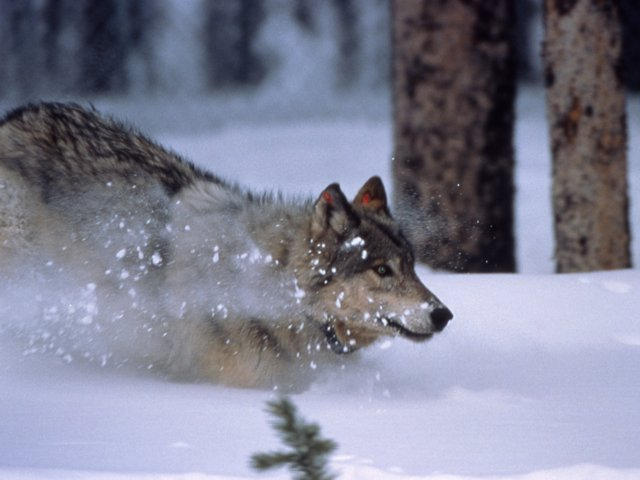
\includegraphics[width=\linewidth]{wolf-snow-1}\\[-1pt]{\scriptsize\color{acGray}волк\par}\end{minipage}\hfill
  \begin{minipage}[t]{0.235\linewidth}\centering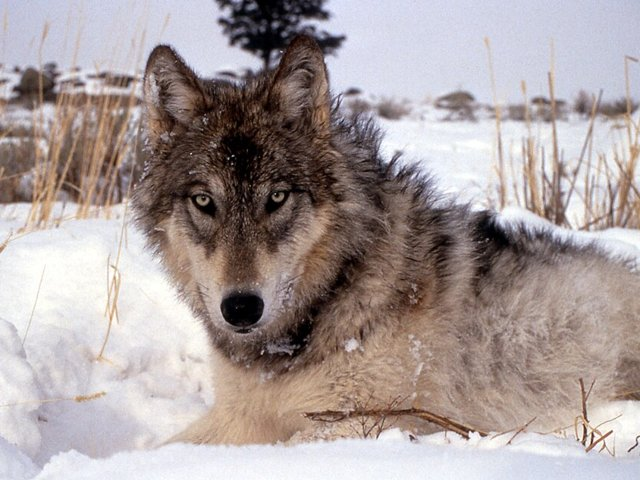
\includegraphics[width=\linewidth]{wolf-snow-2}\\[-1pt]{\scriptsize\color{acGray}волк\par}\end{minipage}\hfill
  \begin{minipage}[t]{0.235\linewidth}\centering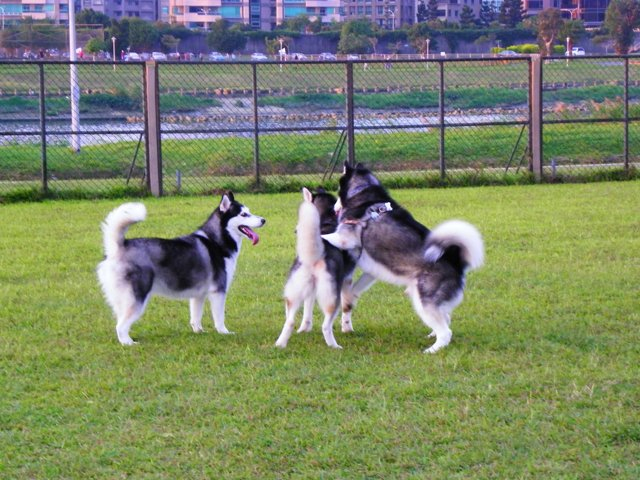
\includegraphics[width=\linewidth]{husky-grass-1}\\[-1pt]{\scriptsize\color{acGray}хаски\par}\end{minipage}\hfill
  \begin{minipage}[t]{0.235\linewidth}\centering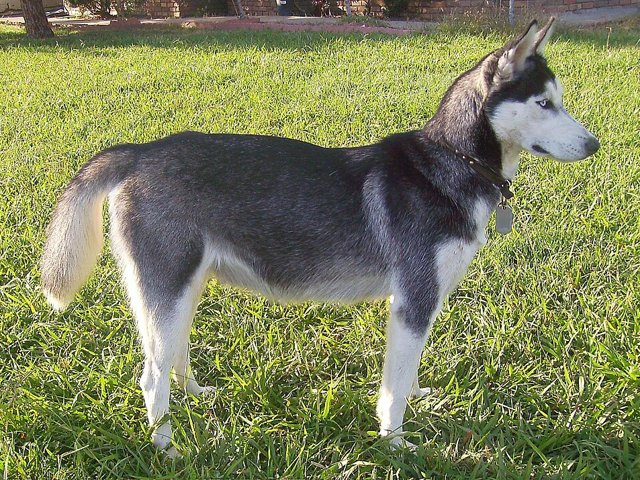
\includegraphics[width=\linewidth]{husky-grass-2}\\[-1pt]{\scriptsize\color{acGray}хаски\par}\end{minipage}

  \medskip
  \raggedright
  \lead{Вопрос.} Точность на отложенной выборке из таких же фото хорошая. Что может пойти не так?

\end{frame}

\begin{frame}[c]{Волк или хаски: ответ}
  \begin{columns}[T]
    \begin{column}{0.40\textwidth}
      \centering
      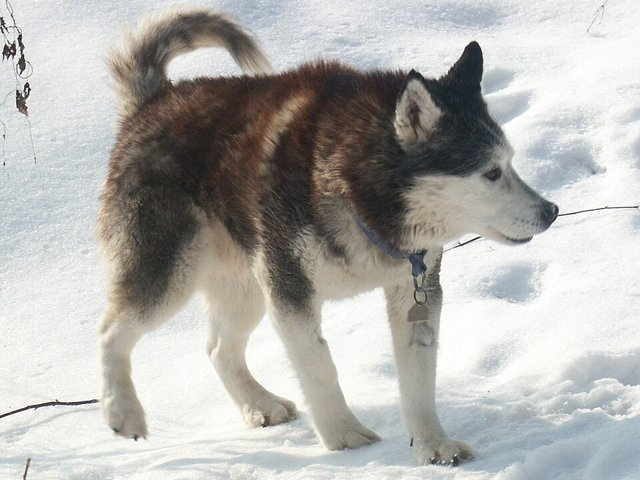
\includegraphics[width=\linewidth]{husky-snow}\\[2pt]
      {\small\color{acOrange}\bfseries Ответ модели: волк\par}
    \end{column}
    \begin{column}{0.54\textwidth}
      \begin{block}{Модель смотрела на снег}
        \small
        Все волки в обучении стояли на снегу, все хаски --- на траве.
        Проще всего отличать их по фону. Хаски на снегу --- «волк».
      \end{block}
      \begin{block}{Эксперимент (2016)}
        \small
        Исследователи специально собрали такую выборку, чтобы показать: высокая точность
        ещё не значит, что модель поняла задачу.
      \end{block}
    \end{column}
  \end{columns}

  \medskip
  \lead{Модель выучит любую закономерность, которая помогает на train,}
  даже если она случайна. Такие проблемы надо ловить при сборе данных.

\end{frame}

\begin{frame}[c]{Задание: собираем датасет листьев}
  \lead{Обсудим вместе.} Хотим, чтобы модель по фото листа определяла дерево.

  \medskip
  \begin{numrows}
    1 & Какие классы? Сколько фото на класс нужно минимум?\\
    2 & Фон, свет, ракурс: одинаковые или разные? Что будет в каждом случае?\\
    3 & Как называть файлы и где хранить ответ (породу)?\\
    4 & Если один лист сфотографирован 5 раз, можно ли эти фото раскидать в train и test?\\
    5 & Как проверить, что другой человек разметил так же?\\
  \end{numrows}
\end{frame}

\begin{frame}[c]{Ответы: правила сбора}
  \begin{columns}[T]
    \begin{column}{0.47\textwidth}
      \begin{block}{Разнообразие}
        \small
        Разные фоны, освещение и телефоны внутри \textbf{каждого} класса.
        Если все клёны сняты на асфальте, а все дубы на траве, модель выучит асфальт.
      \end{block}
      \begin{block}{Баланс}
        \small
        Примерно одинаковое число фото на класс, иначе accuracy обманет.
      \end{block}
    \end{column}
    \begin{column}{0.47\textwidth}
      \begin{block}{Утечка}
        \small
        Фото одного листа --- одна группа. Группа целиком идёт либо в train, либо в test.
        Иначе тест проверяет память, а не умение обобщать.
      \end{block}
      \begin{block}{Единый формат}
        \small
        Инструкция для всех: имя файла, папка класса, таблица с метаданными.
        Тогда датасеты всех учеников можно склеить в один.
      \end{block}
    \end{column}
  \end{columns}
\end{frame}
